\chapter{Derivatives}

In calculus, the derivative of a function represents the rate at which
the function is changing at a particular point. It is a fundamental
concept that has vast applications in various fields, including
physics.\index{derivative}

\section{Definition}

The derivative of a function $f(x)$ at a point $x$ is defined as the limit:

\begin{equation}
f'(x) = \lim_{{h \to 0}} \frac{f(x+h) - f(x)}{h}
\end{equation}

provided this limit exists. In words, the derivative of $f$ at $x$ is
the limit of the rate of change of $f$ at $x$ as the change in $x$
approaches zero.

\section{Applications in Mathematics}
\subsection{l'Hospital's Rule}
Consider the function $h(x) = \frac{\ln{x}}{x-1}$ and suppose we are interested in the behavior of $h(x)$ around $x=1$. If we apply the Quotient Rule, we get an indeterminate result: $$\lim_{x \to 1}\frac{\ln{x}}{x-1} = \frac{0}{0}$$ Looking at the graph of $h(x)$, we can guess that $\lim_{x \to 1}\frac{\ln{x}}{x-1} = 1$. 

\begin{tikzpicture}
\begin{axis}
    [clip=true,
    xmin=0, xmax=4,
    ymin=0, ymax=4,
    axis lines=left
    ]
    \addplot[blue, domain=0.01:4, samples=100]{ln(x)/(x-1)};
    \addplot[samples=50, black, dashed] coordinates{(1, 0)(1,1)};
    \addplot[samples=50, black, dashed] coordinates{(0, 1)(1,1)};
    \addplot[mark=*, fill=white, draw=blue] coordinates{(1, 1)};
\end{axis}
\end{tikzpicture}

Let's examine the numerator and denominator separately: we'll define $f(x)=\ln{x}$ and $g(x) = x-1$. 

\begin{tikzpicture}
    \begin{axis}
    [clip=false,
    xmin=0, xmax=3,
    ymin=-1, ymax=2,
    axis lines = center]
    \addplot[blue, samples=100, domain=1/e:3]{ln(x)}
    node[right, pos=1]{$f(x)$};
    \addplot[red, samples=100, domain=0:3]{x-1}
    node[right, pos=1]{$g(x)$};
    \end{axis}
\end{tikzpicture}

If we zoom in very far around $x=1$, the graphs begin to look linear:

\begin{tikzpicture}
    \begin{axis}
    [clip=false,
    xmin=0.9, xmax=1.1,
    ymin=-0.1, ymax=0.1,
    axis lines = center]
    \addplot[blue, samples=100, domain=0.9:1.1]{ln(x)}
    node[right, pos=0.9]{$f(x)$};
    \addplot[red, samples=100, domain=0.9:1.1]{x-1}
    node[right, pos=1]{$g(x)$};
    \end{axis}
\end{tikzpicture}

We can approximate these graphs as linear functions with slopes $m_1$ and $m_2$, so that the blue curve is approximated as $y=m_1(x-1)$ and the red curve is approximated as $y=m_2(x-1)$. The ratio of the functions would then be $$\frac{m_1(x-1)}{m_2(x-1)}=\frac{m_1}{m_2}$$ which is the same as the ratio of the derivatives of our linear approximations. This suggests l'Hospital's rule, that the limit of a ratio is the same as the limit of the ratio of the derivatives for certain indeterminate forms: $$\lim_{x\to a}\frac{f(x)}{g(x}=\lim_{x\to a}\frac{f'(x)}{g'(x)}$$.

Let's apply l'Hospital's rule to our limit of $h(x)$:
$$\lim_{x\to 1}\frac{\ln{x}}{x-1}=\lim_{x \to 1}\frac{\frac{d}{dx}\ln{x}}{\frac{d}{dx}(x-1)}=\lim_{x \to 1}\frac{\frac{1}{x}}{1}=1$$

Notice our result with l'Hospital's rule matches our guess based on the graph of $h(x) = \frac{\ln{x}}{x-1}$. 

L'Hospital's rule also applies to the indeterminate result $\frac{\pm \infty}{\pm \infty}$. For a limit of the form $\lim_{x\to a}\frac{f(x)}{g(x)}$, l'Hospital's rule applies if:
\begin{enumerate}
    \item the original limit is of the indeterminate form $\frac{0}{0}$ or $\frac{\pm \infty}{\pm \infty}$
    \item $f$ and $g$ are differentiable on an interval containing $a$ (but possibly not differentiable at $a$)
    \item $g'(x) \neq 0$ on said interval
\end{enumerate}

\subsection{Intervals of Increasing and Decreasing Value}
\subsubsection{Practice}
\begin{Exercise}
    [label=incdec1]
    Let $f$ be the function given by $f(x) = 300x-x^3$. On which of the following intervals is $f$ increasing?
\end{Exercise}
\begin{Answer}
    [ref=incdec1]
    First, we will find $f'$ and set it equal to zero: $$f'(x)=300-3x^2=0$$ $$300=3x^2 \rightarrow x=\pm \sqrt{100} = \pm10$$ Now we will evaluate the value of $f'(x)$ for $x<-10$, $-10<x<10$, and $x>10$. 
    \begin{center}
        \begin{tabular}{c|c|c}
        Value of $x$ & Computation & $f(x)$ increasing or decreasing?\\
         $x<-10$    &  $300-3(-11)^2<0$ & decreasing\\
         $-10<x<10$    & $300-3(0)^2>0 $ & increasing\\
         $x>10$&$300-3(11)^2<0$& decreasing
        \end{tabular}
    \end{center}
    Therefore, the fucntion is increasing on the interval $x \in [-10, 10]$ because $f'(x) >0$ for $x \in [-10, 10]$.
\end{Answer}

\subsection{Mean Value Theorem}

The Mean Value Theorem (MVT) states that on an interval $[a, b]$ where a continuous function $f$ is differentiable on an open interval $(a, b)$, there is at least one point where the tangent line to $f$ has the same slope as a line connecting the points $(a, f(a))$ and $(b, f(b))$. Consider the graph of $f(x) = x^2$ below. The line connecting the points $(-1, 1)$ and $(2, 4)$ has a slope of $\frac{1}{2}$. MVT tells us there must be \textit{at least one} point, $c$, on the interval $x \in (-1, 2)$ where $f'(c) = \frac{1}{2}$. We can find this point by setting $f'(x)$ equal to $\frac{1}{2}$: $$2x=\frac{1}{2} \rightarrow x=\frac{1}{4}$$

Examining the graph, you can see that the tangent at $f(\frac{1}{4})$ (the black line) is parallel to the line connecting $(-1, f(-1))$ and $(2, f(2))$. 

\begin{tikzpicture}
    \begin{axis}
        [ymin=-2, xmin=-2, xmax=2, axis lines = left]
        \addplot[blue, samples=50]{x^2};
        \addplot[red, mark=*]coordinates {(-1, 1)};
        \addplot[red, mark=*] coordinates {(2, 4)};
        \addplot[domain=-2:2, red] coordinates{(-1, 1)(2, 4)};
        \addplot[black, mark=*] coordinates{(0.5, 0.25)};
        \addplot[black, domain=-2:2, samples=50
        ]{x-0.25};
    \end{axis}
\end{tikzpicture}

Note that MVT doesn't tell us \textit{where} $f'(x)$ is parallel to the line connecting $(a, f(a))$ and $(b, f(b))$, just that some value $c$ exists that satisfies the condition. 

Consider a hammer thrown upwards at 5 $\frac{m}{s^2}$ on Earth (where the acceleration due to gravity is approximately $-9.8 \frac{m}{s^2}$). We can use MVT to show that there must be some point in the hammer's path upwards where the velocity of the hammer is exactly equal to its average velocity as it flies through the air. 
The hammer's rise can be described with the function $y(t) = 5t-4.9t^2$. The hammer reaches its peak at approximately $t=0.51$. So, we are looking for some value, $c$, such that $$y'(c) = \frac{y(0.51)-y(0)}{0.51-0}=\frac{5(0.51)-4.9(0.51^2)}{0.51}=\frac{1.2755}{0.51}=2.5$$

Solving $y'(t) = 5-9.8t = 2.5$, we find that the $c$ that satisfies MVT is approximately $0.255$. This result is illustrated on the graph below:

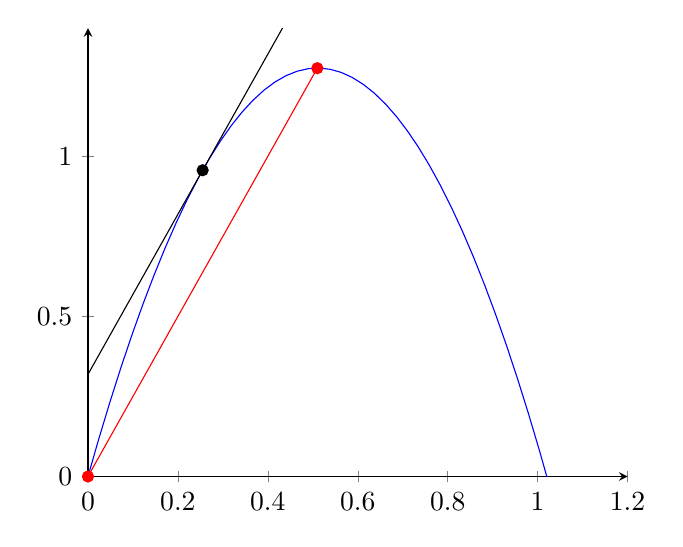
\begin{tikzpicture}
    \begin{axis}[ymin=0,ymax=1.4, xmin=0, xmax=1.2, axis lines=left]
    \addplot[blue, samples=50, domain=0:1.2]{5*x-4.9*x^2};
    \addplot[mark=*, red] coordinates{(0,0)};
    \addplot[mark=*, red] coordinates{(0.51, 1.275)};
    \addplot[red, samples=50]coordinates{(0,0) (0.51, 1.275)};
    \addplot[black, samples=50]{2.5*(x-0.255)+0.9564};
    \addplot[mark=*, black]coordinates{(0.255, 0.9564)};
    \end{axis}
\end{tikzpicture}

\subsubsection{MVT Practice}
\begin{Exercise}
[label=MVT1]
AT 3:30 PM, a car's speedometer reads $30 \frac{mi}{hr}$. At 3:40 PM, it reads $50\frac{mi}{hr}$. Show that at some time between 3:30 and 3:340 PM, the car's acceleration is exactly $120 \frac{mi}{hr^2}$. 
\end{Exercise}
\begin{Answer}
[ref=MVT1]
The speed of a car must a continuous, differentiable function, since your car can't "jump" from one speed to another: it must smoothly accelerate from one speed to another. Therefore, the Mean Value Theorem applies. The average acceleration from 3:30 PM to 3:40 PM is given by:
$$\frac{\text{change in speed}}{\text{change in time}} = \frac{50 \frac{mi}{hr}-30\frac{mi}{hr}}{3:40PM-3:30PM}$$ 
Simplifying and converting minutes to hours, we see the average acceleration is:
$$\frac{20\frac{mi}{hr}}{\frac{1}{6}hr} = 120\frac{mi}{hr^2}$$

Therefore, by MVT, there must be some time between 3:30 and 3:40 PM where the car's acceleration is exactly $120 \frac{mi}{hr^2}$. 
\end{Answer}

\begin{Exercise}
[label=MVT2]
Find the number $c$ that satisfies the MVT on the given interval. 

(a) $f(x) = \sqrt{x}$, $[0, 4]$

(b)$f(x) = e^{-x}$, $[0,2]$

(c)$f(x) = \ln{x}$, $[1,4]$	
\end{Exercise}

\begin{Answer}
[ref=MVT2]
(a) For the domain given, $f(x)$ is defined and differentiable. Finding the slope of the secant line connecting the endpoints:
$$\frac{f(b)-f(a)}{b-a}=\frac{\sqrt{4}-\sqrt{0}}{4-0}=\frac{2}{4}=\frac{1}{2}$$
So we are looking for some number $c$ such that $f'(c) = \frac{1}{2}$. Let's find $f'(x)$:
$$f'(x) = \frac{d}{dx}\sqrt{x}=\frac{1}{2\sqrt{x}}$$
Setting this equal to $\frac{1}{2}$ to find $c$:
$$f'(c) = \frac{1}{2\sqrt{c}}=\frac{1}{2}$$
$$\sqrt{c}=1$$
$$c=1$$

(b)For the domain given, $f(x)$ is defined and differentiable. Finding the slope of the secant line connecting the endpoints:
$$\frac{f(2)-f(0)}{2-0}=\frac{e^{-2}-e^{0}}{2}=\frac{1-e^{2}}{2e^{2}}\approx -0.432$$
And find $f'(x)$:
$$f'(x) = -e^{-x}$$
According to MVT, there must be some $c$ such that $f'(c) \approx-0.432$:
$$-e^{-c} \approx -0.432$$
$$e^{-c}\approx 0.432$$
$$-c \approx \ln{0.432}$$
$$c \approx -\ln{0.432} \approx 0.839$$

(c) For the domain given, $f(x)$ is defined and differentiable. Finding the secant line connecting the endpoints:
$$\frac{f(b)-f(a)}{b-a}=\frac{\ln{4}-\ln{1}}{4-1}=\frac{\ln{4}}{3}\approx 0.462$$
And find $f'(x)$:
$$f'(x) = \frac{1}{x}$$
According to MVT, there must be some $c$ such that $f'(c) \approx 0.462$
$$f'(c) = \frac{1}{c} \approx 0.462$$
$$c \approx \frac{1}{0.462} = 2.164$$
\end{Answer}

\section{Applications in Physics}

In physics, derivatives play a vital role in describing how quantities
change with respect to one another.

\subsection{Velocity and Acceleration}

In kinematics, the derivative of the position function with respect to
time gives the velocity function, and further taking the derivative of
the velocity function gives the acceleration function. For example, if
$s(t)$ represents the position of an object at time $t$, then the
velocity $v(t)$ and acceleration $a(t)$ are given by:

\begin{equation}
v(t) = \frac{ds}{dt} \quad \text{and} \quad a(t) = \frac{dv}{dt} = \frac{d^2s}{dt^2}
\end{equation}

\subsection{Force and Momentum}

In mechanics, the derivative of the momentum of an object with respect
to time gives the net force acting on the object, as stated by
Newton's second law of motion:

\begin{equation}
F = \frac{dp}{dt}
\end{equation}

where $F$ is the force, $p$ is the momentum, and $t$ is the time.

